\iffalse
\documentclass[12pt]{article}
\usepackage{graphicx}
\usepackage{amsmath}
\usepackage{mathtools}
\usepackage{gensymb}
\usepackage{tabularx}
\usepackage{array}
\usepackage[latin1]{inputenc}
\usepackage{fullpage}
\usepackage{color}
\usepackage{array}
\usepackage{longtable}
\usepackage{calc}
\usepackage{multirow}
\usepackage{hhline}
\usepackage{ifthen}
\usepackage{lscape}
\usepackage{float}
\usepackage{amssymb}

\newcommand{\mydet}[1]{\ensuremath{\begin{vmatrix}#1\end{vmatrix}}}
\providecommand{\brak}[1]{\ensuremath{\left(#1\right)}}
\providecommand{\norm}[1]{\left\lVert#1\right\rVert}
\providecommand{\abs}[1]{\left\vert#1\right\vert}
\newcommand{\solution}{\noindent \textbf{Solution: }}
\newcommand{\myvec}[1]{\ensuremath{\begin{pmatrix}#1\end{pmatrix}}}
\let\vec\mathbf

\def\inputGnumericTable{}

\begin{document}
\begin{center}
\textbf\large{OPTIMIZATION}

\end{center}
\section*{Excercise 10.3}


\solution
\fi
The given equation can be written as
\begin{align}
	\label{eq:11/10/3/3/2/conv/eq1}
	\myvec{0&1}\vec{x} &= 2\\
\implies 	\vec{n} &= \myvec{0\\1},\,
	\vec{m} = \myvec{1\\0}
\end{align}
Equation \eqref{eq:11/10/3/3/2/conv/eq1} can be represented in parametric form as
\begin{align}
	\label{eq:11/10/3/3/2/conv/eq2}
	\vec{x} = \vec{A}+\lambda\vec{m}
\end{align}
where
\begin{align}
	\vec{A} &= \myvec{2\\2}.
	\label{eq:11/10/3/3/2/conv/line}
\end{align}
Let $\vec{O}$ be the origin. The perpendicular distance will be the minimum distance from $\vec{O}$ to the line. Let $\vec{P}$ be the foot of perpendicular. This problem can be formulated as an optimization problem as 
\begin{align}
	d &=  \min_{\vec{x}}\norm{\vec{x}-\vec{O}}^2\\
	&=\min_{\lambda}\norm{\vec{A}+\lambda\vec{m}-\vec{O}}^2\\
	&= f\brak{\lambda} = \norm{\vec{m}}^2\lambda^2+2\vec{A}^\top\vec{m}+\norm{\vec{A}}^2
	\label{eq:11/10/3/3/2/conv/eq3}
	\\
	&= \lambda^2+4\lambda+8
\end{align}
$\because$ the coefficient of $\lambda^2>0$, \eqref{eq:11/10/3/3/2/conv/eq3} is convex. 
\begin{align}
	\label{eq:11/10/3/3/2/conv/eq4}
	f^\prime\brak{\lambda} = 2\norm{\vec{m}}^2\lambda+\brak{\vec{A}^\top\vec{m}+\vec{m}^\top\vec{A}}
\end{align}
\begin{enumerate}
\item Computing $\lambda_{min}$ using Derivative method
\begin{align}
	f^{\prime\prime}\brak{\lambda} &= 2\\
	\because f^{\prime\prime}\brak{\lambda}>0,&f^{\prime}\brak{\lambda_{min}}=0, \text{ for } \lambda_{min}\\
	f^{\prime}\brak{\lambda_{min}} &= 2\norm{\vec{m}}^2\lambda_{min}+\brak{\vec{A}^\top\vec{m}+\vec{m}^\top\vec{A}}\\
	\therefore \lambda_{min} &= -\frac{\brak{\vec{A}^\top\vec{m}+\vec{m}^\top\vec{A}}}{2\norm{\vec{m}}^2} = -2
\end{align}
Thus, 
\begin{align}
	\vec{x}_{min} &= \vec{P} = \myvec{2\\2}+\brak{-2}\myvec{1\\0}\\
	&= \myvec{0\\2}\\
	OP &= \norm{\vec{P}-\vec{O}}\\
	&= \norm{\myvec{0\\2}-\myvec{0\\0}}\\
	&= 2
\end{align}
\item Solving using cvxpy, with
\begin{align}
	\vec{n} &= \myvec{0\\1}\\
	\vec{O} &= \myvec{0\\0}\\
	c &= 2\\
	&\min_{\vec{x}}\norm{\vec{x}-\vec{O}}^2 = 2, \vec{x}_{min} = \myvec{0\\2}
\end{align}
\end{enumerate}
See Figs. \ref{fig:11/10/3/3/2/conv/Fig1} and \ref{fig:11/10/3/3/2/conv/Fig2}.
\begin{figure}[!h]
	\begin{center} 
	    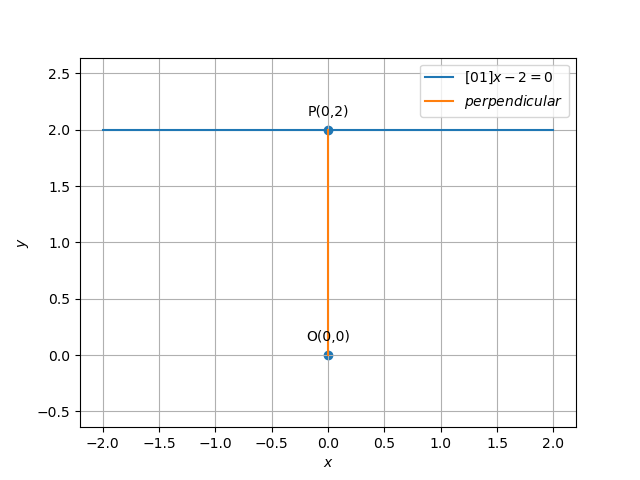
\includegraphics[width=\columnwidth]{11/10/3/3/2/conv/figs/opt1}
	\end{center}
\caption{}
\label{fig:11/10/3/3/2/conv/Fig1}
\end{figure}
\begin{figure}[!h]
	\begin{center} 
	    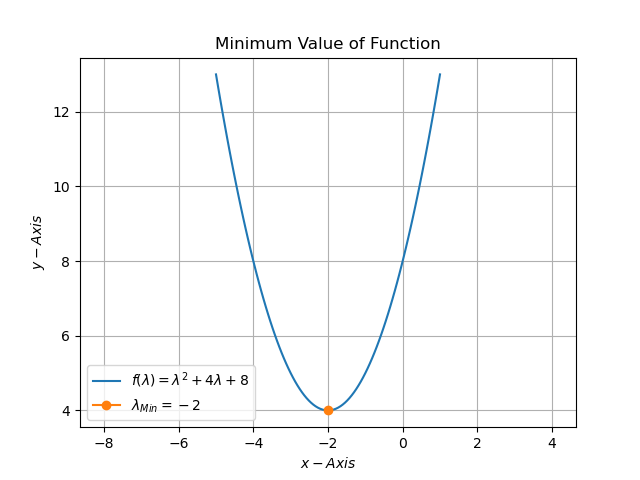
\includegraphics[width=\columnwidth]{11/10/3/3/2/conv/figs/opt2}
	\end{center}
\caption{}
\label{fig:11/10/3/3/2/conv/Fig2}
\end{figure}
